%!TEX root = ../../Main.tex
\graphicspath{{Chapters/Indledning/}}
%-------------------------------------------------------------------------------

\section{Indledning}


\begin{figure}[H]
	\centering
	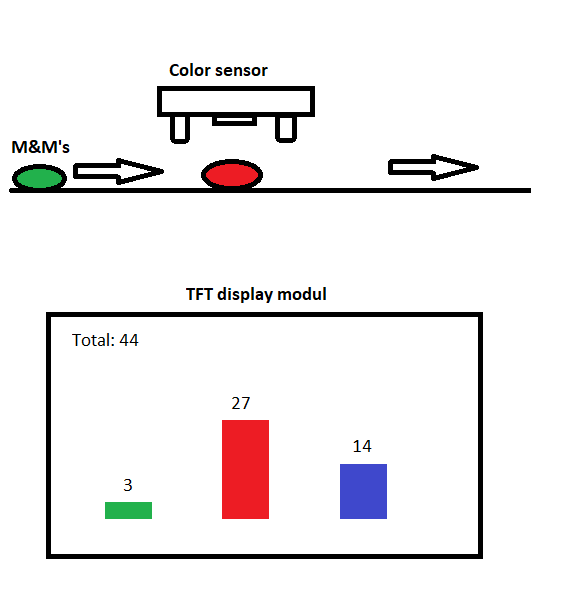
\includegraphics[width = 400pt]{Img/KonceptBillede}
	\caption{Konceptbillede for CSS}
	\label{fig:konceptbillede}
\end{figure}

Color Sorting System(CSS) gør det nemt at sortere diverse emner baseret på deres farve. Disse emner kan være alt fra fødevare til maskin-komponenter, så længe de kan identificeres på farve. CSS fungerer ved at lade emnet passere under en farve sensor, som kan identificere farven på emnet og videresende hvilken farve emnet har til et TFT displaymodul. TFT modulet kan så ved hjælp af søjle diagrammer, fortælle hvor mange forskellige farvet emner der har passeret sensoreren. Resultaterne kan gemmes på et SD kort, hvis man senere skulle bruge dataen. Dog er implementeringen af SD kortet ikke fuldendt i denne prototype, og vil i en viderudvikling af projektet have stor prioritet. Desuden er der kun lagt vægt på color sensor og TFT display modulerne, hvilket vil sige at selve sorteringsmekanikken ikke er implementeret i den nuværende prototype.


\newpage

